\documentclass[aspectratio=169]{beamer}

\usepackage{ccicons}
\usepackage{fontspec}
\usepackage{listings}
\usepackage{tikz}
\usepackage{svg}

\definecolor{uclablue}{RGB}{39,116,174}
\definecolor{uclagold}{RGB}{255,179,0}

\definecolor{ubcorange}{RGB}{158, 66, 37}

\definecolor{cugold}{RGB}{207, 184, 124}
\definecolor{cudarkgray}{RGB}{86, 90, 92}

\definecolor{solarizedred}{RGB}{220, 50, 47}
\definecolor{solarizedblue}{RGB}{38, 139, 210}
\definecolor{solarizedgreen}{RGB}{133, 153, 0}
\definecolor{solarizedpurple}{RGB}{108, 113, 196}
\definecolor{solarizedmagenta}{RGB}{211, 54, 130}

\definecolor{pantone655}{RGB}{0, 42, 92}
\definecolor{pantone7453}{RGB}{123, 164, 217}
\definecolor{pantone633}{RGB}{0, 139, 176}
\definecolor{pantone7492}{RGB}{218, 229, 205}

\colorlet{primarycolor}{pantone655}
\colorlet{secondarycolor}{pantone7453}


\usetikzlibrary{
  arrows,
  arrows.meta,
  automata,
  backgrounds,
  calc,
  chains,
  decorations.pathreplacing,
  fit,
  intersections,
  matrix,
  overlay-beamer-styles,
  positioning,
  shapes,
  shapes.multipart,
  tikzmark,
}
\usetikzmarklibrary{listings}

\hypersetup{
  colorlinks=true,
  urlcolor=cudarkgray,
}

\setbeamercolor{frametitle}{fg=primarycolor}
\setbeamercolor{structure}{fg=primarycolor}
\setbeamercolor{enumerate item}{fg=black}
\setbeamercolor{itemize item}{fg=black}
\setbeamercolor{itemize subitem}{fg=black}

\setbeamersize{text margin left=26.6mm}
\addtolength{\headsep}{2mm}

\setbeamertemplate{navigation symbols}{}
\setbeamertemplate{headline}{}
\setbeamertemplate{footline}{}
\setbeamertemplate{itemize item}{\color{black}}
\setbeamertemplate{itemize items}[circle]

\setbeamertemplate{footline}{
  \begin{tikzpicture}[remember picture,
                      overlay,
                      shift={(current page.south west)}]
    \node [black!50, inner sep=2mm, anchor=south east]
          at (current page.south east) {\footnotesize \insertframenumber};
  \end{tikzpicture}
}

\setsansfont{Inter}[Scale=MatchLowercase]
\setmonofont{Hack}[Scale=MatchLowercase]

\makeatletter
\newcommand\version[1]{\renewcommand\@version{#1}}
\newcommand\@version{}
\def\insertversion{\@version}

\newcommand\lecturenumber[1]{\renewcommand\@lecturenumber{#1}}
\newcommand\@lecturenumber{}
\def\insertlecturenumber{\@lecturenumber}
\makeatother

\setbeamertemplate{title page}
{
  \begin{tikzpicture}[remember picture,
                      overlay,
                      shift={(current page.south west)},
                      background rectangle/.style={fill=pantone655},
                      show background rectangle]
    \node [anchor=west, align=left, inner sep=0, text=white]
          (lecturenumber) at (\paperwidth / 6, \paperheight * 3 / 4)
          {\Large Lecture \insertlecturenumber};
    \node [inner sep=0, align=left, text=white, node distance=0,
          above left=of lecturenumber, anchor=south west, yshift=2mm]
          {\Large ECE 344: Operating Systems};
    \node (title) [inner sep=0, anchor=west, align=left, text=white,
                   text width=30em]
          at (\paperwidth / 6, \paperheight / 2)
          {{\bfseries \Huge \inserttitle{}}};
    \node [inner sep=0, align=right, text=white, node distance=0,
          below right=of title, anchor=north east, yshift=-1mm]
          {{\footnotesize \ttfamily \insertversion}};
    \node [inner sep=0, text=white, align=left, anchor=west]
          (author) at (\paperwidth / 6, \paperheight / 4)
          {\insertauthor};
    \node [text=white, inner sep=0, align=left, node distance=0,
           below left=of author, anchor=north west, yshift=-2mm]
          {\insertdate};
    \node [align=right, anchor=south east, inner sep=2mm, text=white]
          (license) at (\paperwidth, 0)
          {\footnotesize This  work is licensed under a
           \href{http://creativecommons.org/licenses/by-sa/4.0/}
                {\color{pantone7453} Creative Commons Attribution-ShareAlike 4.0
                 International License}};
    \node [text=white, inner sep=0, align=right, node distance=0,
           above right=of license, anchor=south east, xshift=-2mm]
          {\Large \ccbysa};
  \end{tikzpicture}
}

\tikzset{
  >=Straight Barb[],
  shorten >=1pt,
  initial text=,
}

\lstset{
  basicstyle=\footnotesize\ttfamily,
  language=C,
  escapechar=@,
  commentstyle=\color{black!50},
}


\lecturenumber{28}
\title{Hard Disk Drives}
\version{1.0.0}
\author{Jon Eyolfson}
\date{November 27, 2022}

\begin{document}
  \begin{frame}[plain, noframenumbering]
    \titlepage
  \end{frame}

  \begin{frame}{The Structure of a Hard Disk Drive (aka HDD)}
    \begin{center}
        \includegraphics[height=0.8\textheight]{hdd1.png}
    \end{center}
  \end{frame}

  \begin{frame}{Access Speed Depends on Locality}

    Sectors on same track can be read continuously

    \vspace{2em}

    Switching tracks needs repositioning of the arm

    \hspace{2em} Repositioning the arm is expensive)
  \end{frame}

  \begin{frame}{You Physically Address a HDD Using Cylinder-Head-Sector (CHS)}

    Data has the following Coordinates (multi-dimensional polar coodinates):

    \begin{itemize}
      \item Platter: which revolving platter (addressed as head) [z Axis]
      \item Track: which track lane on platter (historically cylinder) [$||r||$]
      \item Sector: which sector on track [$\Theta$]
    \end{itemize}

    \vspace{2em}

    The historical CHS has an approximate 8 GB limit of addressable space

    \hspace{2em} (512 bytes/sector)×(63 sectors/track)×(255 heads (tracks/cylinder))

    \hspace{2em} ×(1024 cylinders)

    \vspace{2em}

    LBA (Logical Block Addressing) uses one number to address

    any block and is not limited to 8~GB
  \end{frame}

  \begin{frame}{Shingled Magnet Recording (SMR)}

    The write head only writes in the center of a track, and has unused padding

    \vspace{2em}

    You can't write to this padding without destroying neighboring tracks

    \vspace{2em}

    SMR however, allows you to write over the padding, if you do it sequentially

    \vspace{2em}

    Drive performance may suffer, but it's easier to increase capacity 

    \includegraphics[height=20mm]{hdd2.png}
  \end{frame}

  \begin{frame}{HDDs Have Latencies Dependent on the Distance Travelled}

    Rotational delay: physically rotate the disk to get to the correct sector

    \hspace{2em} Typically 4-8 ms (average delay is half of a full rotation)

    \vspace{2em}

    Seek time: moving the disk arm to get to the correct track

    \hspace{2em} Typically 0.5-2 ms

    \vspace{2em}

    Transfer time: how long it takes to read bytes from the disk

    \hspace{2em} Typically the maximum transfer speed is 125 MB/s
  \end{frame}

  \begin{frame}{Calculating Transfer Rate}

    The total time, $\mathsf{T}$, is equal to

    \hspace{2em} rotational delay + seek time + transfer time

    \vspace{2em}

    The transfer rate, $\mathsf{R}$, is equal to

    \hspace{2em} Size of the transfer / $\mathsf{T}$

    \vspace{2em}

    What is the transfer rate of

    \hspace{2em} Large sequential accesses?

    \hspace{2em} Small random accesses?
  \end{frame}

  \begin{frame}{We Should Use HDDs Sequentially Whenever Possible}
    \begin{tabular}{lll}
                       & HDD 1     & HDD 2      \\
      Rotational speed & 7,200 RPM & 15,000 RPM \\
      Rotational latency (ms) & 4.2 & 2.0 \\
      Average seek (ms) & 9 & 4 \\
      Max transfer & 105 MB/s & 125 MB/s \\
      Platters & 4 & 4 \\
      Interface & SATA & SCSI \\
    \end{tabular}

    \vspace{2em}

    Sequential 100 MB read:

    \hspace{2em} HDD 1, T = 950 ms, R = 105 MB/s

    \hspace{2em} HDD 2, T = 800 ms, R = 125 MB/s

    Random 4 KB read:

    \hspace{2em} HDD 1, T = 13.2 ms, R = 0.31 MB/s

    \hspace{2em} HDD 2, T = 6 ms, R = 0.66 MB/s
  \end{frame}

  \begin{frame}{Logical Mapping Could Place All Sectors Next to Each Other}

    \begin{center}
    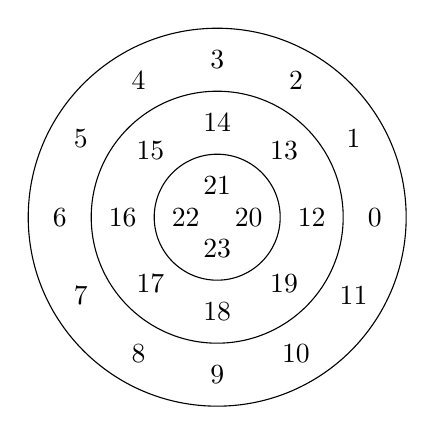
\begin{tikzpicture}
      \draw (0,0) circle (2.4cm);
      \draw (0,0) circle (1.6cm);
      \draw (0,0) circle (0.8cm);
      \foreach \i in {0,1,...,11}
      {
        \draw (\i*360/12: 2cm) node {\i};
      }
      \foreach \i in {12,13,...,19}
      {
        \draw (\i*360/8 - 180: 1.2cm) node {\i};
      }
      \foreach \i in {20,21,...,23}
      {
        \draw (\i*360/4: 0.4cm) node {\i};
      }
    \end{tikzpicture}
    \end{center}

    You may want to offset the sectors in different tracks so the head has
    time to settle

    \hspace{2em} Track skew allows the disk to be efficient with minimal head
    movement
  \end{frame}

  \begin{frame}{You May Want More Flexibility Than the Default Mapping}
    Pros

    \hspace{2em} Simple to program

    \hspace{2em} Default mapping reduces seek time for sequential access

    \vspace{2em}

    Cons

    \hspace{2em} Filesystem can't inspect or try to optimize the mapping

    \hspace{2em} Trying to reverse the mapping is difficult

    \hspace{4em} Number of sectors per track changes

    \hspace{4em} Disk silently remaps bad sectors
  \end{frame}

  \begin{frame}{A Cache Can Significantly Speed Up Disk Transfers}

    Disks have some internal memory (WD Red - 64 MB) for caching

    \vspace{2em}

    Implement a read-ahead ``track buffer''

    \hspace{2em} Read the entire contents of the track into memory during the rotational delay

    \vspace{2em}

    Write caching with volatile memory

    \hspace{2em} Write back: claim data is written to disk

    \hspace{4em} Fast, but there's data loss if there's a power failure

    \hspace{4em} Write through: acknowledge after data is physically written
  \end{frame}


  \begin{frame}{We Can Schedule Disk Accesses}

    We want to minimize the time the disk moves without reading or writing data

    \vspace{2em}

    FCFS: schedule requests in the order received

    \hspace{2em} Fair, but it has a high seek and rotation cost

    \vspace{2em}

    SSTF: shortest seek time first

    \hspace{2em} Handle the nearest cylinder/sector next

    \hspace{4em} Pro: reduces arm movement (seek time)

    \hspace{4em} Con: unfair, can starve some requests
  \end{frame}

  \begin{frame}{Elevator (aka SCAN or C-SCAN) Sweeps Across the Disk}
    \begin{center}
    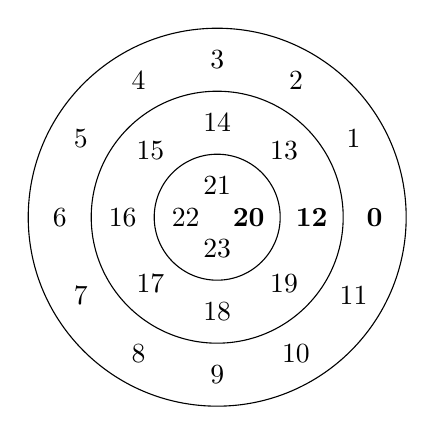
\begin{tikzpicture}
      \draw (0,0) circle (2.4cm);
      \draw (0,0) circle (1.6cm);
      \draw (0,0) circle (0.8cm);
      \draw (0: 2cm) node {\bf 0};
      \draw (0: 1.2cm) node {\bf 12};
      \draw (0: 0.4cm) node {\bf 20};
      \foreach \i in {1,...,11}
      {
        \draw (\i*360/12: 2cm) node {\i};
      }
      \foreach \i in {13,...,19}
      {
        \draw (\i*360/8 - 180: 1.2cm) node {\i};
      }
      \foreach \i in {21,...,23}
      {
        \draw (\i*360/4: 0.4cm) node {\i};
      }
    \end{tikzpicture}
    \end{center}

    If a request comes in for a track already serviced this sweep, queue it for
    the next
  \end{frame}

  \begin{frame}{Elevator (or SSTF) Ignores Rotation}
    \begin{center}
    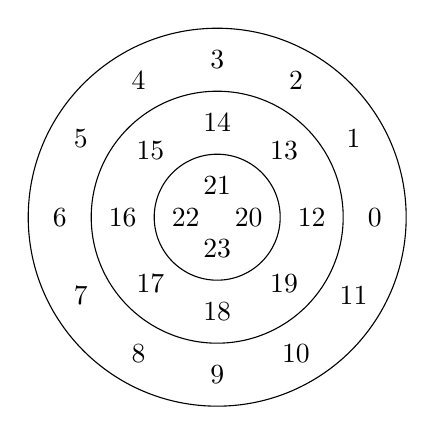
\begin{tikzpicture}
      \draw (0,0) circle (2.4cm);
      \draw (0,0) circle (1.6cm);
      \draw (0,0) circle (0.8cm);
      \foreach \i in {0,1,...,11}
      {
        \draw (\i*360/12: 2cm) node {\i};
      }
      \foreach \i in {12,13,...,19}
      {
        \draw (\i*360/8 - 180: 1.2cm) node {\i};
      }
      \foreach \i in {20,21,...,23}
      {
        \draw (\i*360/4: 0.4cm) node {\i};
      }
    \end{tikzpicture}
    \end{center}

    Shortest positioning time first (SPTF) is often the best strategy

    \hspace{2em} The OS and disk need to work together to implement this
  \end{frame}

  \begin{frame}{Disks Enable Persistence}

    We explored two HDDs today:
    \begin{itemize}
      \item Magnetic disks have poor random access (need to be scheduled)
      \item Shortest Positioning Time First (SPTF) is the best scheduling for throughput
    \end{itemize}
  \end{frame}

\end{document}
